
\begin{figure}[H]
  {
    \setlength{\tabcolsep}{3.0pt}
    \setlength\cmidrulewidth{\heavyrulewidth} % Make cmidrule = 
    \begin{adjustbox}{width=3cm,center}
      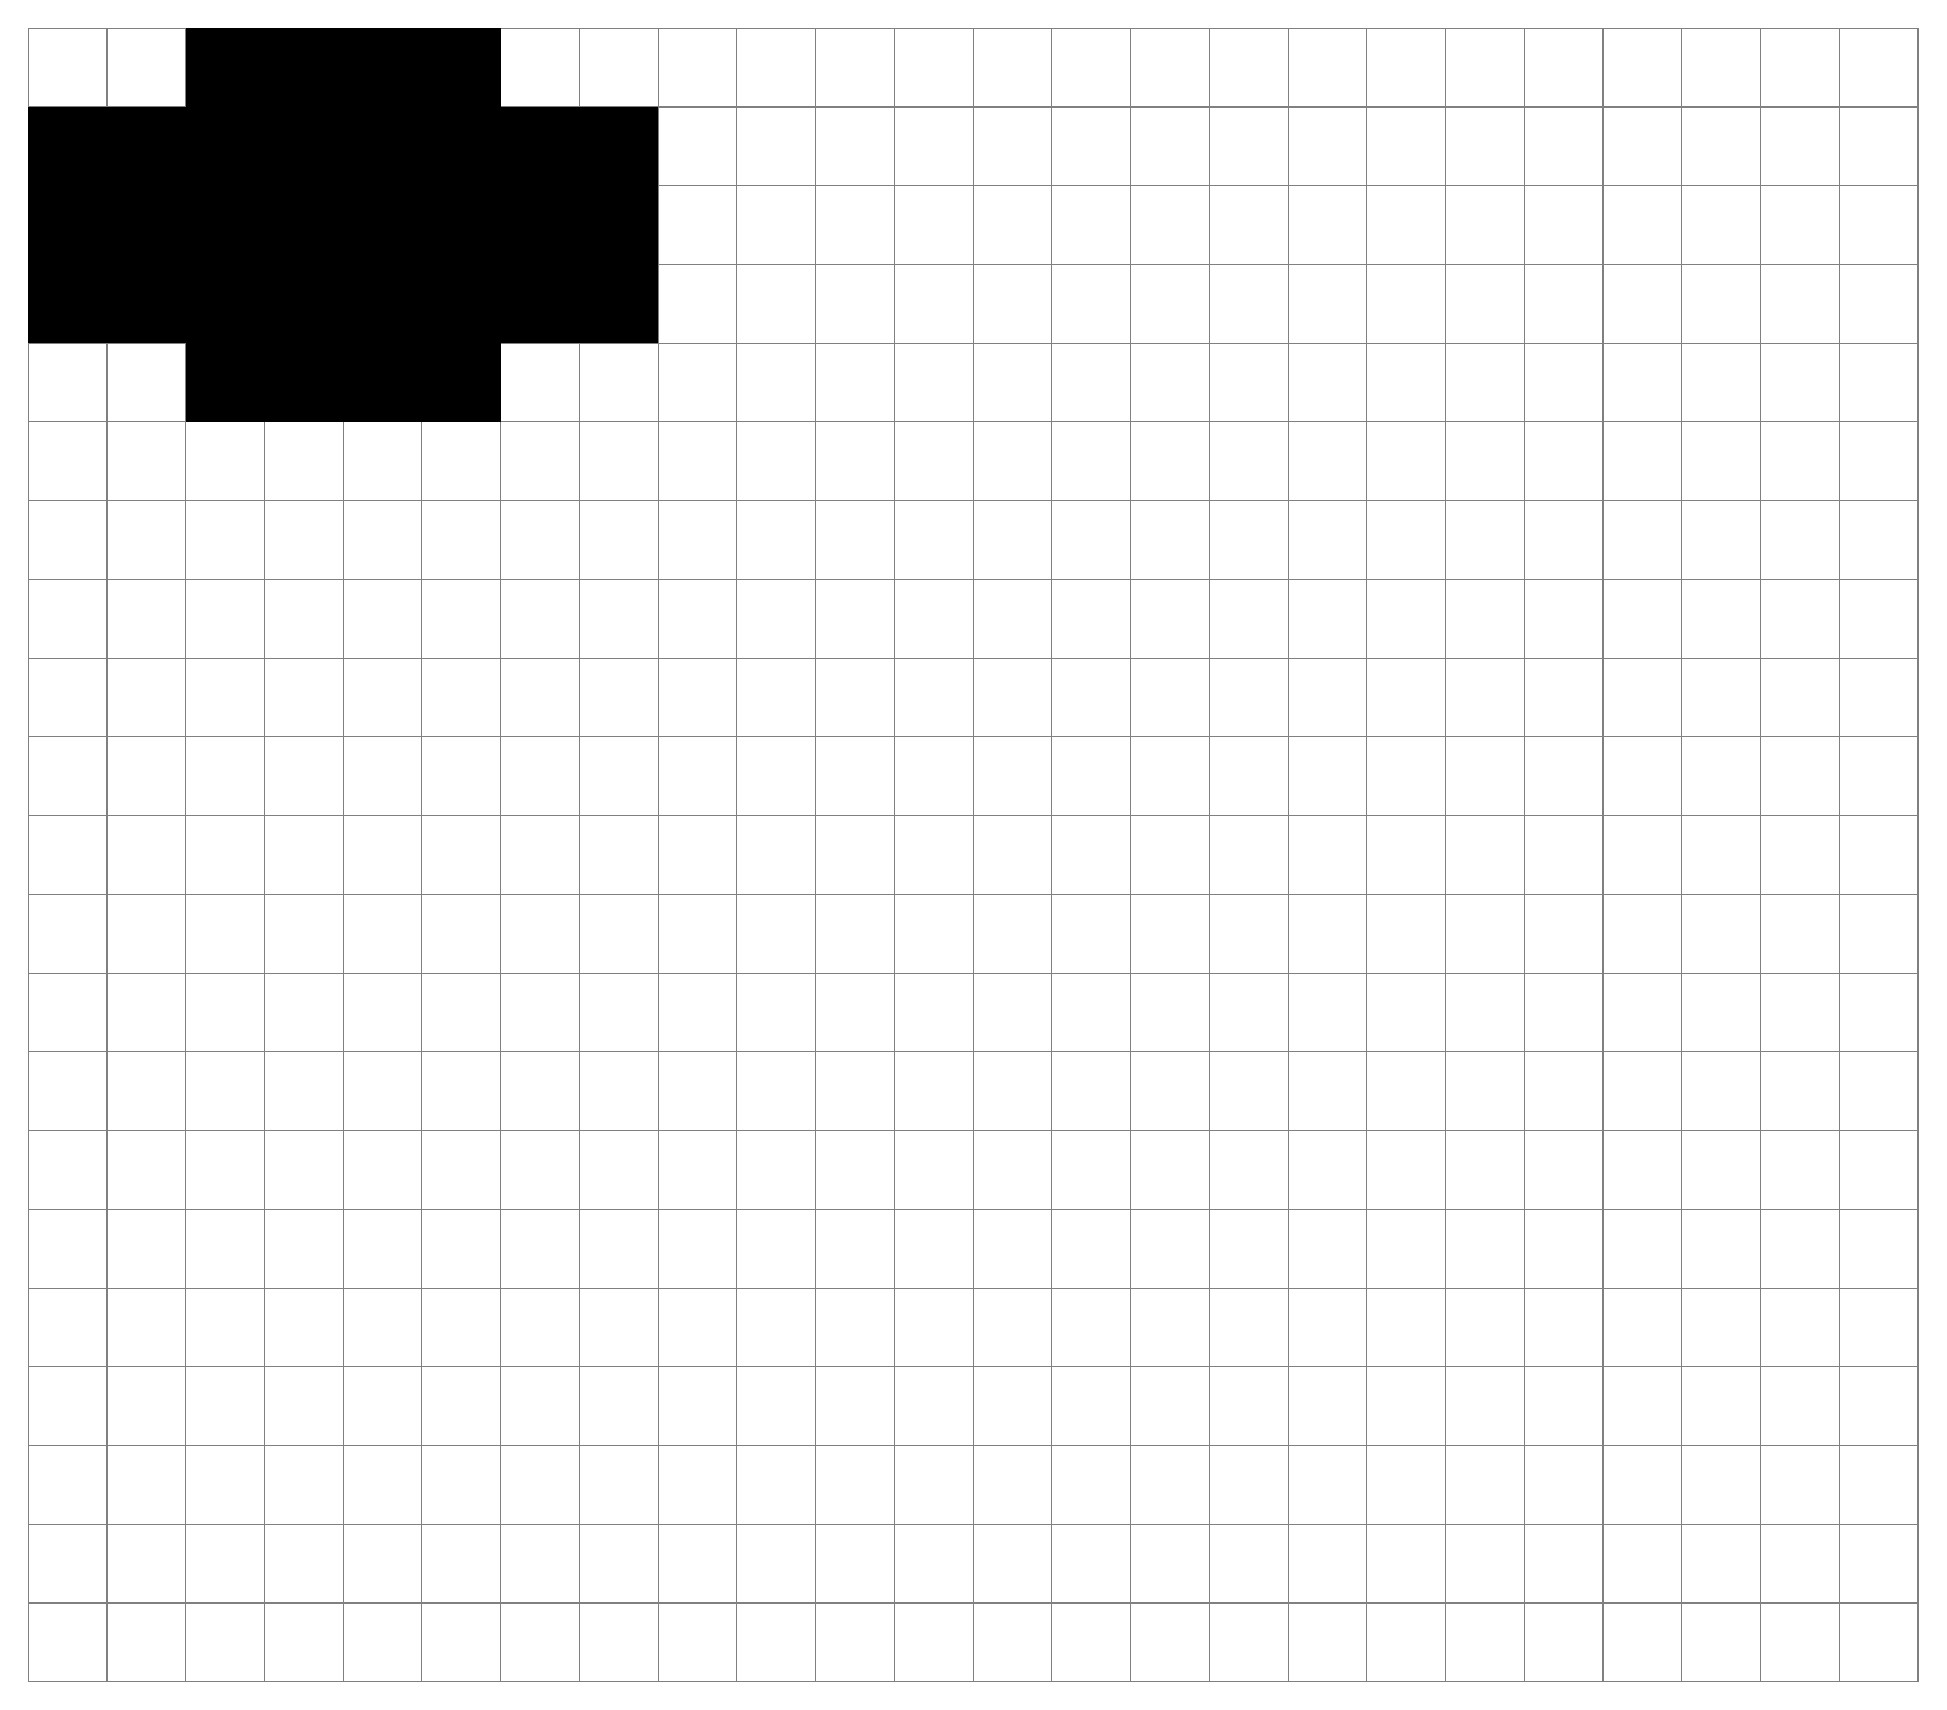
\begin{tikzpicture}

	\draw[step=1.0,gray,thin] (0,0) grid (24,21);
	\fill[\MULTICOLORTWO] (2,20) rectangle ++ (1,1);
	\fill[\MULTICOLORTWO] (3,20) rectangle ++ (1,1);
	\fill[\MULTICOLORTWO] (4,20) rectangle ++ (1,1);
	\fill[\MULTICOLORTWO] (5,20) rectangle ++ (1,1);
	\fill[\MULTICOLORTWO] (0,19) rectangle ++ (1,1);
	\fill[\MULTICOLORTWO] (1,19) rectangle ++ (1,1);
	\fill[\MULTICOLORONE] (2,19) rectangle ++ (1,1);
	\fill[\MULTICOLORONE] (3,19) rectangle ++ (1,1);
	\fill[\MULTICOLORONE] (4,19) rectangle ++ (1,1);
	\fill[\MULTICOLORONE] (5,19) rectangle ++ (1,1);
	\fill[\MULTICOLORTWO] (6,19) rectangle ++ (1,1);
	\fill[\MULTICOLORTWO] (7,19) rectangle ++ (1,1);
	\fill[\MULTICOLORTWO] (0,18) rectangle ++ (1,1);
	\fill[\MULTICOLORTWO] (1,18) rectangle ++ (1,1);
	\fill[\MULTICOLORTWO] (2,18) rectangle ++ (1,1);
	\fill[\MULTICOLORTWO] (3,18) rectangle ++ (1,1);
	\fill[\MULTICOLORTWO] (4,18) rectangle ++ (1,1);
	\fill[\MULTICOLORTWO] (5,18) rectangle ++ (1,1);
	\fill[\MULTICOLORTWO] (6,18) rectangle ++ (1,1);
	\fill[\MULTICOLORTWO] (7,18) rectangle ++ (1,1);
	\fill[\MULTICOLORTWO] (0,17) rectangle ++ (1,1);
	\fill[\MULTICOLORTWO] (1,17) rectangle ++ (1,1);
	\fill[\MULTICOLORONE] (2,17) rectangle ++ (1,1);
	\fill[\MULTICOLORONE] (3,17) rectangle ++ (1,1);
	\fill[\MULTICOLORONE] (4,17) rectangle ++ (1,1);
	\fill[\MULTICOLORONE] (5,17) rectangle ++ (1,1);
	\fill[\MULTICOLORTWO] (6,17) rectangle ++ (1,1);
	\fill[\MULTICOLORTWO] (7,17) rectangle ++ (1,1);
	\fill[\MULTICOLORTWO] (2,16) rectangle ++ (1,1);
	\fill[\MULTICOLORTWO] (3,16) rectangle ++ (1,1);
	\fill[\MULTICOLORTWO] (4,16) rectangle ++ (1,1);
	\fill[\MULTICOLORTWO] (5,16) rectangle ++ (1,1);

      \end{tikzpicture}
    \end{adjustbox}
  }\caption{SMALLDOT}
\end{figure}
